% !TeX root = ../main.tex
\section{Исследование динамического диапазона, свободного от побочных составляющих (SFDR)}

Динамический диапазон, свободный от побочных составляющих (SFDR --- Spurious-Free Dynamic Range), характеризует отношение мощности основного полезного колебания к мощности максимальной паразитной гармоники в рабочей полосе частот:
\begin{equation}
    \text{SFDR} = 10 \lg \left( \frac{P_{\text{осн}}}{P_{\text{поб,макс}}} \right) = P_{\text{осн}}[\text{дБ}] - P_{\text{поб,макс}}[\text{дБ}],
    \label{eq:sfdr_def}
\end{equation}
где:
\begin{itemize}
    \item $P_{\text{осн}}$ --- мощность полезного монохроматического сигнала на промежуточной частоте ($f_{IF} = 0.1$ МГц);
    \item $P_{\text{поб,макс}}$ --- мощность наибольшей побочной (паразитной) дискретной спектральной составляющей в пределах исследуемой полосы частот;
    \item $P_{\text{осн}}[\text{дБ}]$ и $P_{\text{поб,макс}}[\text{дБ}]$ --- спектральные уровни соответствующих составляющих, выраженные в логарифмическом масштабе (дБ).
\end{itemize}

В цифровом гетеродине (ЦГ) ограниченная разрядность тригонометрических таблиц отсчетов приводит к возникновению периодической погрешности аппроксимации синусоиды, формирующей дискретные паразитные гармоники в спектре. На рисунке \ref{fig:sfdr_bits} приведена полученная зависимость SFDR от разрядности сетки цифрового гетеродина ($nobg$) при фиксированной разрядности входного АЦП ($noba = 13$ бит).

\begin{figure}[H]
    \centering
    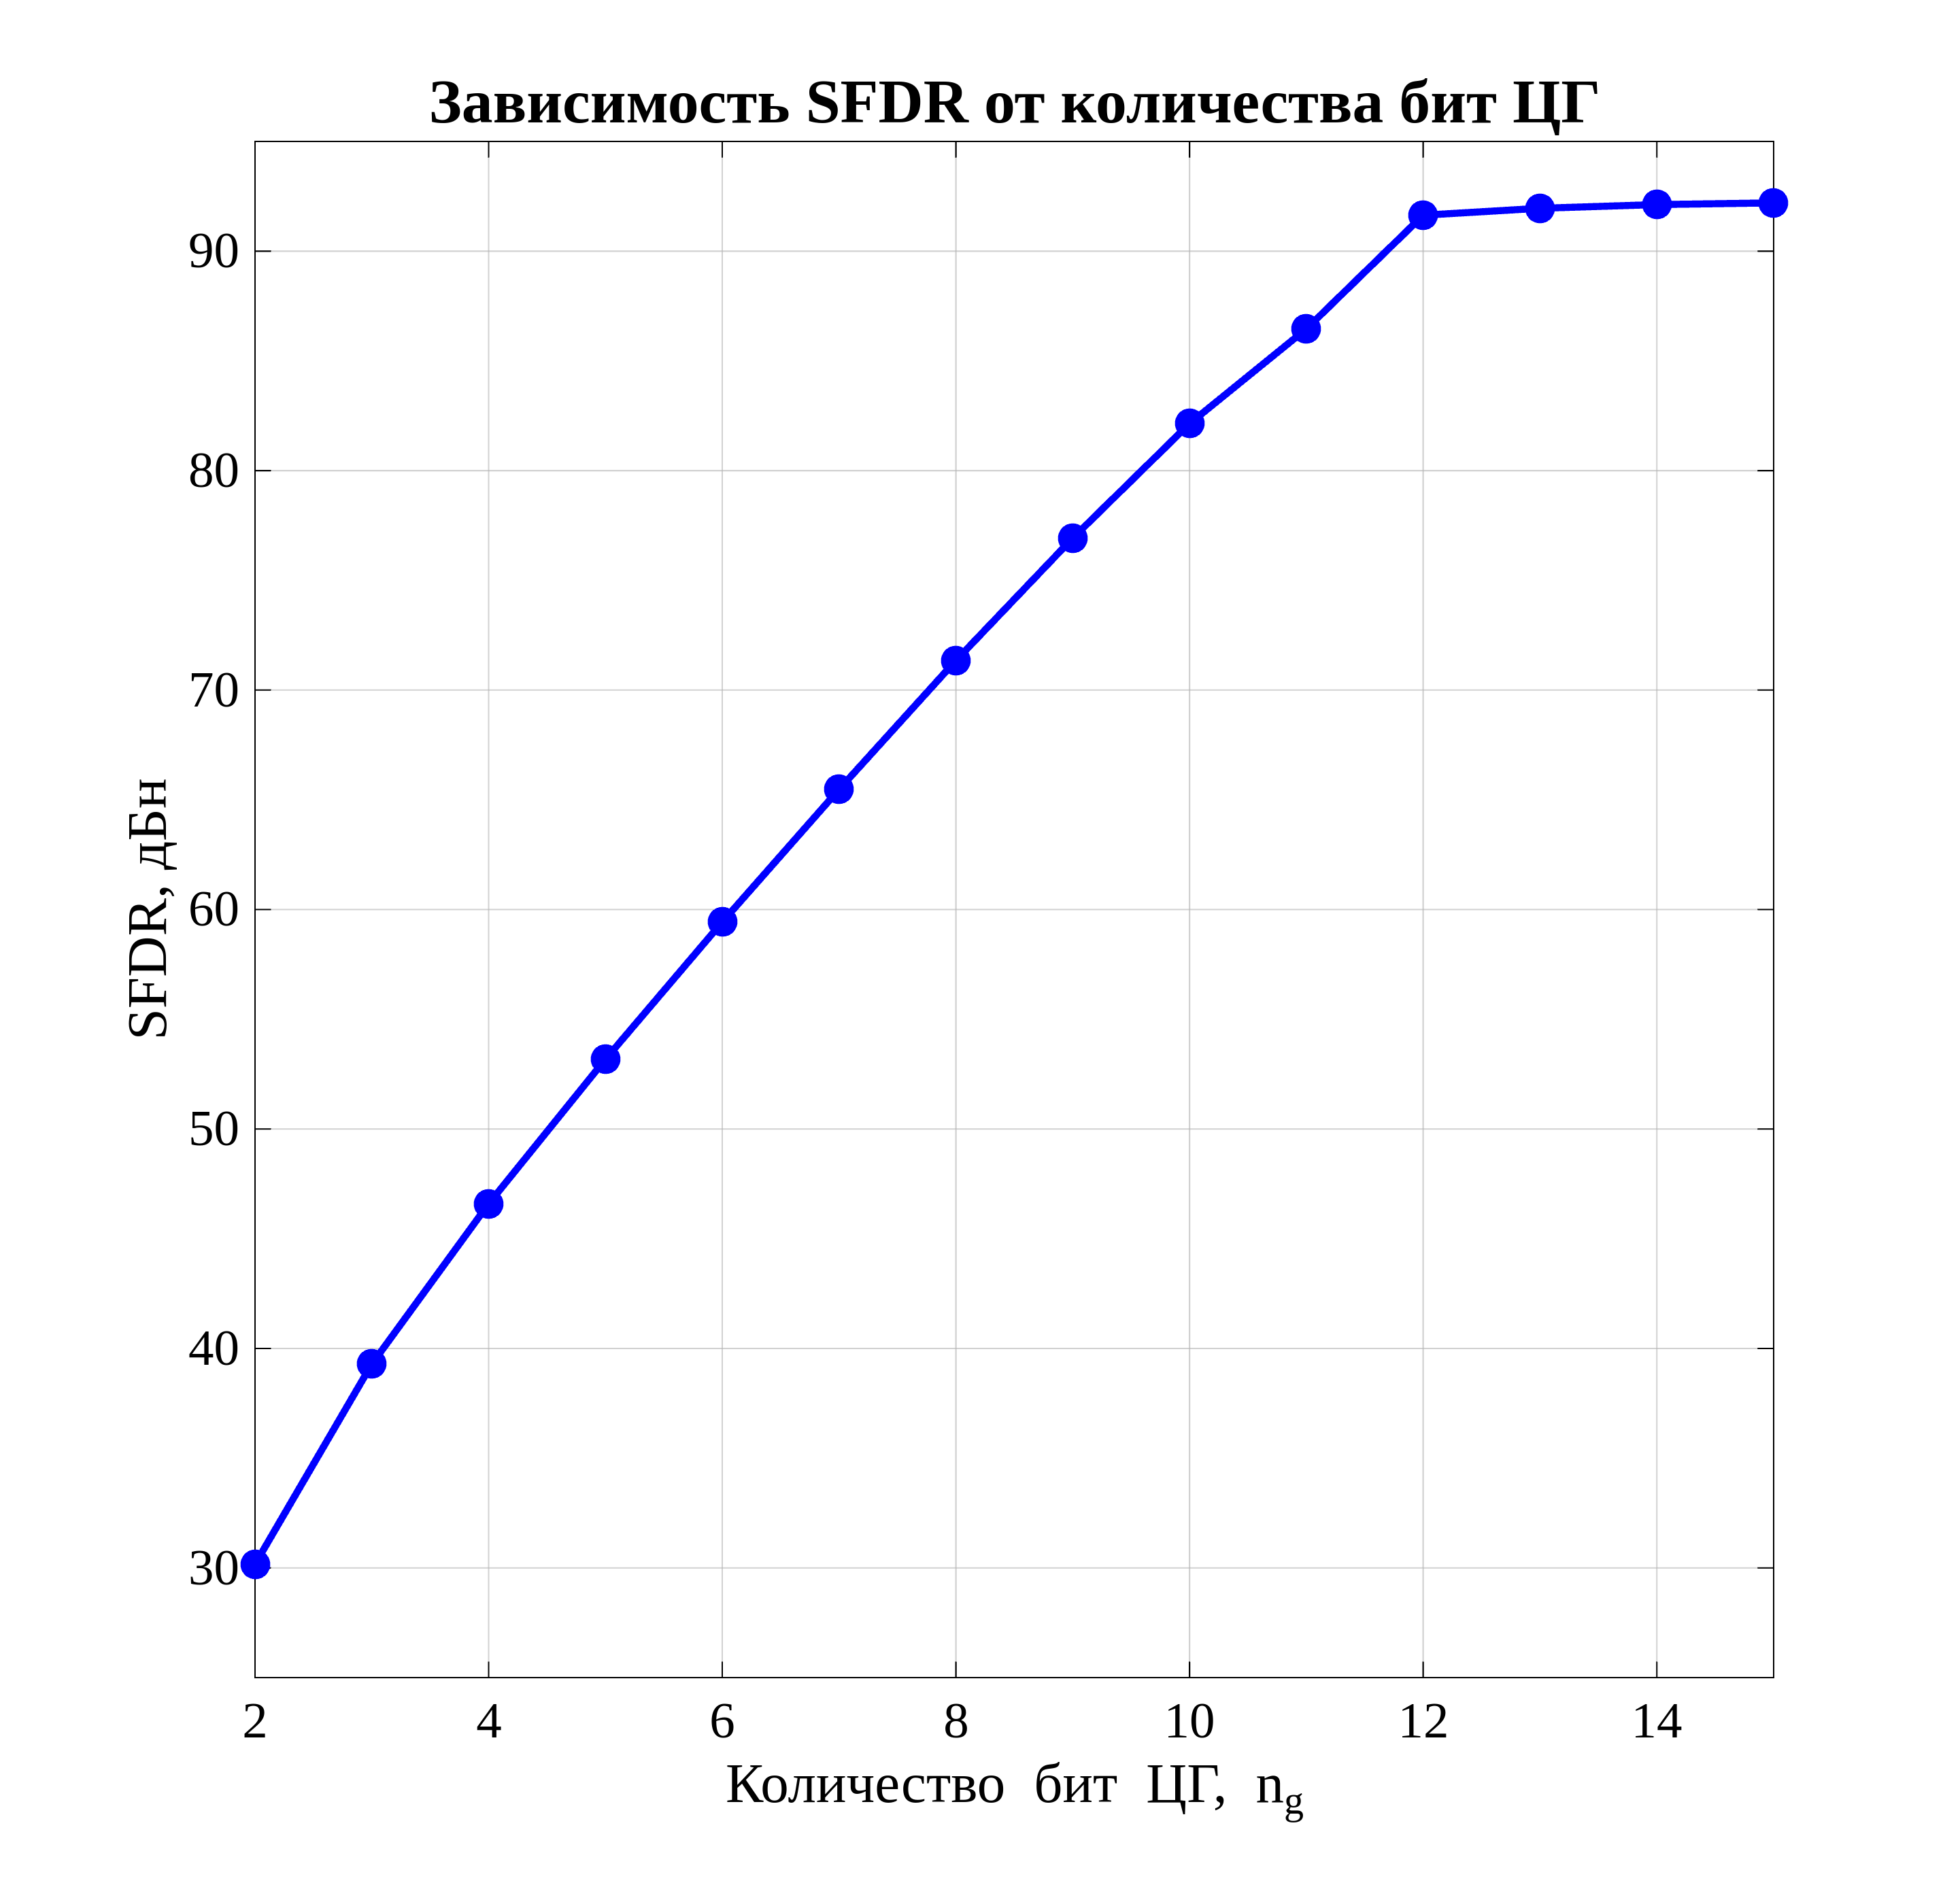
\includegraphics[width=0.7\textwidth]{export_figs/p3_sfdr_vs_bits.png}
    \caption{Зависимость динамического диапазона SFDR от разрядности ЦГ}
    \label{fig:sfdr_bits}
\end{figure}

Анализ полученной зависимости показывает:
\begin{enumerate}
    \item В области малой разрядности ($nobg < 13$ бит) наблюдается устойчивый линейный рост динамического диапазона с увеличением числа бит. В этой зоне динамический диапазон тракта лимитируется исключительно побочными гармониками округления самого гетеродина.
    \item При достижении разрядности $nobg \ge 13$ бит характеристика выходит на постоянный уровень (область насыщения). Побочные составляющие ЦГ опускаются ниже порога шумов входного АЦП ($noba = 13$ бит) и заданного шума смеси, поэтому дальнейшее усложнение разрядной сетки гетеродина не приводит к росту SFDR.
\end{enumerate}
